\documentclass[task=1]{exercise}
\usepackage{enumitem}
\usepackage{schule}
\usepackage{harpoon}

\usepackage{tikz}
\usepackage{circuitikz}

\newcommand\SJ{Schuljahr 22/23}

\newcommand\makeGlobalHeader[4]{
  \setgroup{#1\\#2}
  \settitle[#4]{#3}
  \addstudent{Datum:}
  \addstudent{~}
}

\newcommand\stufe{Wiederholung}
\newcommand\topic{Mathematik}

\newcommand\makeHeader[2]{
  \makeGlobalHeader{\topic}{\stufe}{#1}{#2}
}


\makeHeader{Naturphänomene Elektrostatik}{Faraday'scher Käfig}

\renewcommand{\vec}{\overrightharp}

\begin{document}
  Bei einem Gewitter, sagt man, ist man im Auto vor eintreffenden Blitzen geschützt, weil dieses ein sogenannter Faraday'scher Käfig ist. Warum ist das so und was genau ist ein Faraday'scher Käfig?
  
  Jede geschlossene Hülle aus einem elektrischen Leiter ist ein Faraday'scher Käfig. Um herausfinden, warum uns diese vor eintreffenden Blitzen schützt, müssen wir zwei Fälle unterscheiden:
  \begin{enumerate}[label=\textnormal{\arabic*)}]
   \item Warum sind wir im Auto vor einem Blitzeinschlag direkt in uns geschützt?
   \item Was passiert beim Blitzeinschlag ins Auto/in den Faray'schen Käfig? Gefährlich sind für uns Menschen vorallem die großen Ströme, die bei einem Blitzeinschlag fließen können. Wo fließen hier welche Ströme?
  \end{enumerate}
  Diese Fragen wollen wir uns nun näher anschauen.

  \task[Warum bin ich im Auto vor einem direkten Blitzeinschlag geschützt?]
  \begin{enumerate}
  \item In der Abbildung ist ein Leiter zwischen zwei geladenen Polen dargestellt. Zeichne ein, wie sich die freien Ladungsträger verhalten und benenne das elektrostatische Phänomen.\\~\\
  Man nennt dieses elektrostatische Phänomen: \luecke{4cm}.
  \begin{center}
    \vspace{.5cm}
    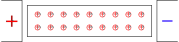
\includegraphics[width=.5\textwidth]{images/influenceSimple.pdf}
    \vspace{.5cm}
  \end{center}
  

  \item Nun siehst du einen leitenden Ring zwischen zwei geladenen Platten.
  \begin{center}
    \vspace{.5cm}
    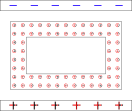
\includegraphics[width=.5\textwidth]{images/influenceFaraday.pdf}
    \vspace{.5cm}
  \end{center}
    \begin{enumerate}[label=\textnormal{\arabic*)}]
    \item\label{item:capField} Zeichne zuerst die Feldlinien mit einer Farbe deiner Wahl ein, die zwischen den geladenen Platten entstehen würden, wenn der leitende Ring {\bfseries nicht} da wäre.
    \item\label{item:infl} Zeichne nun ein, wie sich die frei beweglichen Ladungsträger im Ring verhalten.
    \item\label{item:faraday} Wähle nun eine andere Farbe als bei Aufgabe \ref{item:capField} und zeichne die Feldlinien ein, die entstehen, wenn man ausschließlich die verschobenen Ladungsträger im leitenden Ring aus Aufgabe \ref{item:infl} betrachtet.
    \item Welche Schlüsse ziehst du aus dem entstandenen Bild in Aufgabe \ref{item:faraday}?\\~\\
    \begin{minipage}[t]{.45\linewidth}
      Nutze deine Erkenntnis, um zu erklären, was im hier abgebildeten Grießkorn-Versuch passiert:
    \end{minipage}
    \hfill
    \begin{minipage}[t]{.4\linewidth}
    \vspace{.1cm}
    \includegraphics[width=\linewidth]{images/faradayGriess.png}
    \end{minipage}\\
    \vspace{1cm}
  \end{enumerate}
  \item In einer Gewitterwolke kommt es zu einer sehr starken Ladungstrennung zwischen dem oberen Teil der Wolke und der unteren. Das Ergebnis ist, dass sich im unteren Teil der Gewitterwolke sehr viele negative Ladungsträger sammeln.
  \begin{enumerate}[label=\textnormal{\arabic*)}]
  \item Ausgehend davon, dass die Erde ein elektrischer Leiter ist, wie heißt das Phänomen, dass du auf der Erdoberfläche (lokal unter der Gewitterwolke) beobachten wirst?
  Benenne das Phänomen und erkläre kurz, was passiert.\\\vspace{2cm}
  \item\label{item:WolkeErde}
  \begin{minipage}[t]{.5\linewidth}
   Mach eine Skizze von der Wolke und der Erdoberfläche, in der du jeweils die Ladung der überschüssigen Ladungsträger kennzeichnest (\glqq +\grqq~oder \glqq --\grqq) und die Feldlinien einzeichnest. Nimm für die Feldlinien an, dass es sich bei Wolke und Erde jeweils um zwei geladene Platten handelt. Achte jedoch auf die Regeln zum Zeichnen der Feldlinien.
  \end{minipage}\\
  \vspace{1cm}
  \item
  \begin{minipage}[t]{.5\linewidth}
   Mach eine Skizze wie in Aufgabe \ref{item:WolkeErde}, zeichne aber nun auch ein Auto ein und kennzeichne die Feldlinien. Die Frage, warum du vor direktem Blitzeinschlag sicher bist, kannst du beantworten, wenn du bedenkst, dass der Blitz nur dort einschlagen kann, wo Feldlinien beginnen oder enden.
  \end{minipage}
  \end{enumerate}
  \end{enumerate}
  
  \newpage
  \task[Welche Ströme fließen beim Blitzeinschlag ins Auto?]
  Wir machen eine einfache Überschlagsrechnung.\\
  \begin{minipage}[t]{.65\linewidth}
      Bei einem Blitzeinschlag kann ein kurzzeitiger Strom $I_0$ von bis zu $100.000\,\mathrm{A}$ fließen. Für uns Menschen wird es bei Gleichstrom ab ca. 120\,mA gefährlich.\\
      Nehmen wir an, dass der elektrische Widerstand eines Menschen von beiden Händen bis zu beiden Füßen $600\,\mathrm{\Omega}$ beträgt.\\
      Wir nehmen weiterhin an, dass der Mensch im Auto während des Blitzeinschlages mit beiden Händen an das (nicht-isolierte) Dach fässt und mit beiden Füßen den unverkleideten Boden des Autos berührt (siehe Skizze).
    \end{minipage}
    \hfill
    \begin{minipage}[t]{.3\linewidth}
    \vspace{.1cm}
    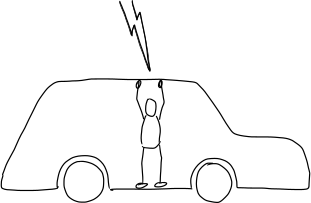
\includegraphics[width=\linewidth]{images/MenschImAuto.pdf}
    \end{minipage}\\~\\~\\
  Über die Karosserie des Autos nehmen wir an, dass sie komplett aus Stahl besteht (wie bei den Autos aus den 80er Jahren). Nach einer einfachen Überschlagsrechnung\footnote{Stahl hat einen spezifischen Widerstand von etwa $0{,}1\,\frac{\mathrm{\Omega\cdot mm^2}}{\mathrm{m}}$. Nehmen wir an, dass die Karosserie ca. 2\,mm dick ist, der Umfang des Autos etwa 5\,m beträgt und seine Höhe etwa 1\,m, so kommen wir auf einen elektrischen Widerstand der Seitenfläche der Karosserie von etwa $10^{-5}\,\mathrm{\Omega}$\,. Nehmen wir weiterhin an, dass das Dach und die Bodenfläche einen ähnlichen Beitrag zum Widerstand leisten, so erhalten wir einen Gesamtwiderstand von $3\cdot 10^{-5}\,\mathrm{\Omega}$\,.\\ An dieser Näherung kann man vieles verbessern. Hast du eine Idee, wie zum Beispiel?} nehmen wir an, dass die Karosserie einen Gesamtwiderstand von $3\cdot 10^{-5}\mathrm{\Omega}$ hat.\\
  Somit ergibt sich folgendes Ersatzschaltbild:\\~\\
  \begin{minipage}[t]{.45\linewidth}
  \vspace{.01cm}
  \begin{circuitikz}[european, voltage shift=0.5]
 \draw (0,3) node[anchor=east] {}
 to[short, o-*, f=$I_0$] (2,3)
 to[R=$~600\,\mathrm{\Omega}$, f>_=$I_1$] (2,0);
 \draw (2,3) -- (4,3)
 to[R=$~3\cdot 10^{-5}\,\mathrm{\Omega}$, f>_=$I_2$]
 (4,0) to[short, -o] (0,0);
 \end{circuitikz}
 \end{minipage}
 \hfill
  \begin{minipage}[t]{.45\linewidth}
    ~\\~\\Berechne ausgehend vom Ersatzschaltbild den Strom $I_1$, der durch den Menschen fließt.
  \end{minipage}
\end{document}
